\subsection{Search Algorithms Used in CrowdHTN}
\label{improv: search algorithms}
As part of the re-engineering of CrowdHTN, we changed the implementation of the search algorithms to be based on a fringe. As mentioned in \cite{holler2020htn} we can simply switch out the underlying fringe data structure to emulate different search algorithms without making any changes to our core planner. Enabled by this change, we have implemented four search algorithms and will discuss them in the following section:
\begin{itemize}
	\item Random depth-first search
	\item Random breadth-first search
	\item Greedy best-first search
	\item A-star like search
\end{itemize}
\begin{comment}
	- as mentioned in \cite{holler2020htn}, we can use a fringe-based implementation of progression search to swap out the fringe and realize different search strategies
	- the old implementation of Crowd did not properly do this, but we switched the implementation to allow us to test different algorithms here
\end{comment}

\subsubsection{Random Depth-First Search}
Randomized depth-first search is the only search algorithm that was already present in the previous implementation of CrowdHTN. It is implemented using a Last-In-First-Out queue as our fringe. Whenever new search nodes are inserted into the fringe we randomize their order to keep the random properties of the original CrowdHTN. This is done to avoid any pathological cases where e.g. the first method applicable to a task leads to an endless loop. We do not expect any differences in behavior or performance compared to the previous implementation.

\subsubsection{Random Breadth-First Search}
Randomized breadth-first search is the first new search algorithm that we implemented. It is done by using a First-In-First-Out queue, allowing us to explore all the potential task hierarchies layer by layer. The insertion order of new nodes is randomized as in the depth-first-search. We do this as the number of search nodes may be exponential in the depth, e.g. if each task can be resolved by at least two reductions. \todo{Get more detailed here?} As such, the order in which we explore the nodes of any layer may still have a big impact and in this way we avoid pathological behavior. \\
In general, we expect a higher memory footprint compared to depth-first search and assume that the planner will struggle with domains where either plans are only found in deep layers or where the branching factor is very high as both will lead to a blowup in the size of our queue. At the same time, we expect the performance of breadth-first search to be a lot more consistent than for depth-first search, as the layer at which we find a plan stays fixed for any single instance. \\
Overall, we do not expect high performance of our breadth-first search. It may however prove useful on some domains and help us understand and validate assumptions about the behavior of TOHTN problems.
\begin{comment}
- expect more memory
- worse performance
- will struggle with high branching factor or deep plans

- trivially complete, will always encounter everything
- reference statistics (branching factor from Crowd, minimal plan depth from Lilotane) to show that 

- probably not the best performance
- will help validate assumptions about TOHTN characteristics
\end{comment}

\subsubsection{Heuristic Search}
Both depth-first and breadth-first search are unguided and do not depend the order of search node exploration on any information contained in those nodes. Other planners, such as PANDA, use heuristics to guide their search. We will describe general information about heuristics and their use in PANDA according to \cite{holler2020htn} and then describe how we try and adapt the use of heuristics for malleable TOHTN planning.

\paragraph{Heuristics in HTN in general and PANDA specifically}
\label{improv: crowd heuristic}
The general idea of heuristics is to avoid exploring all of our search space. They achieve this by guiding the search to the most promising search nodes first.
In TOHTN planning, our choices during search are restricted by both the hierarchy of tasks as well as the world state. As a result, the best heuristics should make use of both pieces of information for the best results. \\
One avenue to deriving heuristics for HTN planning would be to adapt classical planning heuristics. This proves difficult, however, as these heuristics do not know about the hierarchy and may assume a state-based goal which HTN planning often does not have. To avoid such issues, the PANDA planner goes the other way around. PANDA computes a classical planning problem which is a relaxation of the HTN problem at hand. Then a solution to this relaxed model is approximated with the help of classical planning heuristics and the result is used to guide the initial HTN planning procedure. The computation of the classical model is possible in polynomial time and only done fully in the beginning, afterwards the model is only updated for the current state of planning. As a result, the heuristic takes into account both hierarchy and world state while remaining relatively efficient.
\begin{comment}
\cite{holler2020htn} (PANDA GBFS)
- heuristics allow us to not explore all of the search space
- hierarchy and world state both restrict our search, we should consider both, makes heuristic design difficult
- classical planning heuristics have problems:
- ignore the hierarchy
- heuristics have state-based goals, HTN not necessarily
- relax the HTN problem to classical planning (heuristic!) -> relaxed composition model
- uses actions and state of HTN problem
- adds reachability information
- then use another classical planning heuristic to solve the relaxed model
- use the resulting distance for HTN

- simplifications of the transformation:
- can use tasks that are not part of the decomposition hierarchy
- ordering constraints in decompositions are ignored
- each task task can only be introduced once and is then 'shared' in a way
- the size of the heuristic model is linear in the size of the input problem P
- computing the heuristic model is in $\mathcal{P}$
- update the model while searching

- heuristic is based on a grounded model
\end{comment}

\paragraph{Problems with the PANDA heuristic for malleable HTN planning}
While PANDA has managed to make great use of heuristics in HTN planning, we cannot simply adopt the same heuristics for malleable CrowdHTN. The reason for this lies in the assumption of PANDA that a ground problem instance is already available. Grounding is an expensive operation, though, as discussed in \cite{behnke2020succinct}. A full grounding may be exponential in size compared to the input and run times of grounding and can be accordingly high. \\
While such a grounding is already available in PANDA, CrowdHTN does not perform explicit grounding before planning. Doing so may prove interesting for a parallel planner where the grounding would only be performed once. In a malleable environment without shared memory we can expect this grounding to take place every time a new worker is added, adding a high startup cost. Worse, a short-lived worker may be interrupted while still grounding, never getting around to any planning work. This would interfere with the efficient usage of available resources. For this reason we have decided against using the PANDA heuristics in CrowdHTN and instead tried to design a simpler heuristic to be used in malleable TOHTN planning.
\begin{comment}
- PANDA and its heuristics are great
- however, this imposes a startup cost
- implicitly assume a fully grounded instance (up to exponential size!)
- depending on instance grounding can take multiple minutes! (even for the efficient PANDA grounder up to 40 seconds)
- we perform this work multiple times, especially in a malleable environment
\end{comment}
\paragraph{A Heuristic for Malleable HTN Planning}
\todo{argue admissibility of our heuristic?}
To counter the startup cost of the PANDA heuristic, we have devised a simpler heuristic which is cheap to precompute and can easily be used in malleable planning. The goal is to have little startup overhead and to retain the efficient evaluation at each planning step. While this necessarily limits any precomputation to the lifted instance and the precision of our heuristic comes with problems as discussed in the previous paragraphs, we hope to still find some performance gains on at least some problem instances. \\
As heuristic value, we use a lower bound on the number of reductions we still need to perform to fully resolve our list of open tasks. When computing this lower bound we ignore preconditions and effects, searching the shortest possible way through the hierarchy. We precompute this value for each task as described in algorithm \ref{algo: gbfs heuristic}. The remaining depth for each action is initialized to zero. The remaining depth for each abstract task is initially unknown. In each step we loop over all tasks $t$ whose remaining depth is unknown. For each method $m$ of task $t$ we check the depth of all subtasks. If all depths are known, the method depth is set to the sum of all subtask depths plus one. For each task we choose the minimum value over all available reductions. \\
If in any iteration we do not get a new depth for at least one task, we stop the computation. Any task which does not have an assigned depth at this point is not resolvable at all and can be ignored. \\
Let $t_a$ be the set number of abstract tasks, $t_p$ be the number of primitive tasks and $m$ the number of methods. A single iteration takes time in $\mathcal{O}(t_a + m)$. The number of overall iterations required is bound by $t_a$, as in any iteration at least one abstract task will be assigned it's final score, as we do not have any negative cycles. This gives us an overall runtime bound of $\mathcal{O}(t_p + t_a \cdot(t_a + m))$. As all those numbers are relating to the lifted instance we expect the overall run time to be small in practice.
\begin{comment}
- inspired by PandaGBFS
- GBFS:
	- use a heuristic to grade each node
	- next node: best of all neighbors of the current node
	- then do a DFS on this
- GBFS is not complete
- might get stuck in an infinite loop
\todo{Quote to describe GBFS?}

The heuristic:
- use a heuristic that is cheap in both preprocessing and in computation during each step
- determine the minimum number of actions/ reductions needed to solve the task network
- ignore any and all parameters and world state to simplify the computation
\todo{ensure the code actually does this!}
- iterative approach:
	- initial:
		- actions have remaining depth 0
		- reductions without children/ where all children are noops have depth 1
	- iterating:
		- reductions: the sum of the minimum depths of all subtasks + 1
		- tasks: the minimum over all reductions
- i.e., we heuristically try to find nodes with the minimum amount of work remaining
- each iteration gives us the remaining depth of at least 1 compound task, else we terminate
- i.e., efficient to compute
- tasks that do not receive a value are unresolvable and can be pruned
\end{comment}
\begin{algorithm}
	\caption{GBFS heuristic calculation}
	\label{algo: gbfs heuristic}
	task depths $\gets \{(t_c, 0) | t_c \in \text{ concrete tasks}\}$\;
	\While{task depths changed}{
		% get reduction depths
		\For{$t_c \in$ compound tasks}{
			reduction depths $= \emptyset$\;
			\For{$r \in$ reductions for $t_c$}{
				\If{depths of all subtasks are known}{
					reduction depths $\cup= 1 + \sum \{d | d \text{ is depth of a subtask of } r \}$\;
				}
			}
			
			\If{reduction depths $\neq \emptyset$}{
				task depths $\cup= \{ (t_c, \min (\text{reduction depths})) \}$\;
			}
		}
	}
\end{algorithm}
To evaluate our heuristic while planning, we now need to look not only at one but at the whole sequence of open tasks and calculate the sum of our heuristic over those tasks. While the naive solution gives us linear runtime in the number of open tasks, we can stretch the computation over task instantiation and reuse parts of it to perform heuristic evaluation in $\mathcal{O}(1)$ at run time.
\cite{refer to implementation chapter - we build up the sum as we instantiate new search nodes}
Additionally, while we only use this heuristic to guide TOHTN planning, it ignores any orderings between open tasks. As such, it can be applied to HTN planning as well.

\paragraph{Using the new heuristic in TOHTN planning}
With the new heuristic presented in the previous paragraph, we implemented two new search algorithms for CrowdHTN, those being a guided depth-first search and an A-star like search. \\
The implementation of depth-first search used so far performs the search in a uniformly random order. Without knowing anything about the domain, this is a reasonable choice. While it is far from optimal search, it also avoids any pathological cases that may arise from a fixed order of exploration. As an alternative to this random order, we used the heuristic to guide our depth-first search. We have to note that this is still not necessarily deterministic. Randomness comes into play both when two reductions have the same heuristic score - which happens for different instantiations of the same method - and when performing work stealing in a parallel setting. \\
In addition to the guided depth-first search, we also implemented an A-star like search where a node's value is the sum of the heuristic value and the number of applied reductions. We differ from A-star in that we terminate the search as soon as a plan has been found instead of continuing on the search for an optimal plan. The hope is that the heuristics guide us towards a plan while giving weight to the number of applied reductions forces us to turn back and explore other parts of the search space without getting lost in pathological cases.

\subsubsection{Completeness of different Search Algorithms}
\label{improv: search completeness}
In the previous paragraphs we discussed a number of different search algorithms that we implemented for CrowdHTN and how we expect them to effect the performance characteristics of our planner. The search algorithm has a more fundamental impact than that, however, and may effect the property of completeness. In this section we want to give a short overview over the completeness of each of the algorithms. A short overview can be seen in table \ref{table: search completeness}. Note that this discussion is only about the algorithms without any modifications. In section \ref{improv: loop detection} we discuss loop detection mechanisms to improve those algorithms which are so far not listed as complete. \\
\begin{table}
	\caption{Completeness of the different search algorithms in CrowdHTN}
	\label{table: search completeness}
	\centering
	\begin{tabular}{| l | l |}
		\hline
		Algorithm & Completeness Property \\
		\hline
		Random DFS & Not complete. Positive probability to find a plan if it exists \\
		Random BFS & Complete \\
		Heuristic DFS & Incomplete \\
		A-star like & Complete \\
		\hline
	\end{tabular}
\end{table}
Depth-first search is not complete as it may enter an endless loop and, even if it still explores side-tracks from this loop, will never be able to backtrack to before the start of this loop, cutting of parts of the search space. There is however always a chance to find a plan if it exists. I.e., there is a non-zero chance that the random choices all happen to be done correctly and the goal is found even if other paths may lead into endless loops. \\
Breadth-first search on the other hand is trivially complete. While the exploration order within each layer is random we can provide an upper bound on the number of steps required to explore a given search node $n$ on layer $i$. One such bound is the sum of all layer sizes from 0 up to and including $i$. \\
Next in our list is heuristic depth-first search. Similar to random depth-first search it may run into an endless loop. Compared to depth-first search, however, heuristic depth first search may do so in a deterministic fashion if the domain triggers a pathological case in the heuristic. One example domain which would trigger such a case in our heuristic is visualized in figure \ref{figure: improv heuristic pathological}. Here rectangles stand for tasks, rounded rectangles for actions and arrows to reductions. Assume we want to resolve task $t_1$ where the preconditions of $m_1$ do not hold while those of $m_2, m_3, m_4, m_5$ are fulfilled. Our heuristic will want us to resolve $t_1$ via $m_1$ which does not work. Then the next shortest path to a full resolution is through $m_2, m_1$. $m_2$ will be applied successfully to recurse, $m_1$ will fail again and the cycle continues like this forever. The path through $m_3, m_4, m_5$ has length 3 and will thus never be taken. \\ 
\begin{figure}
	\caption{A pathological case in our new HTN heuristic}
	\label{figure: improv heuristic pathological}
	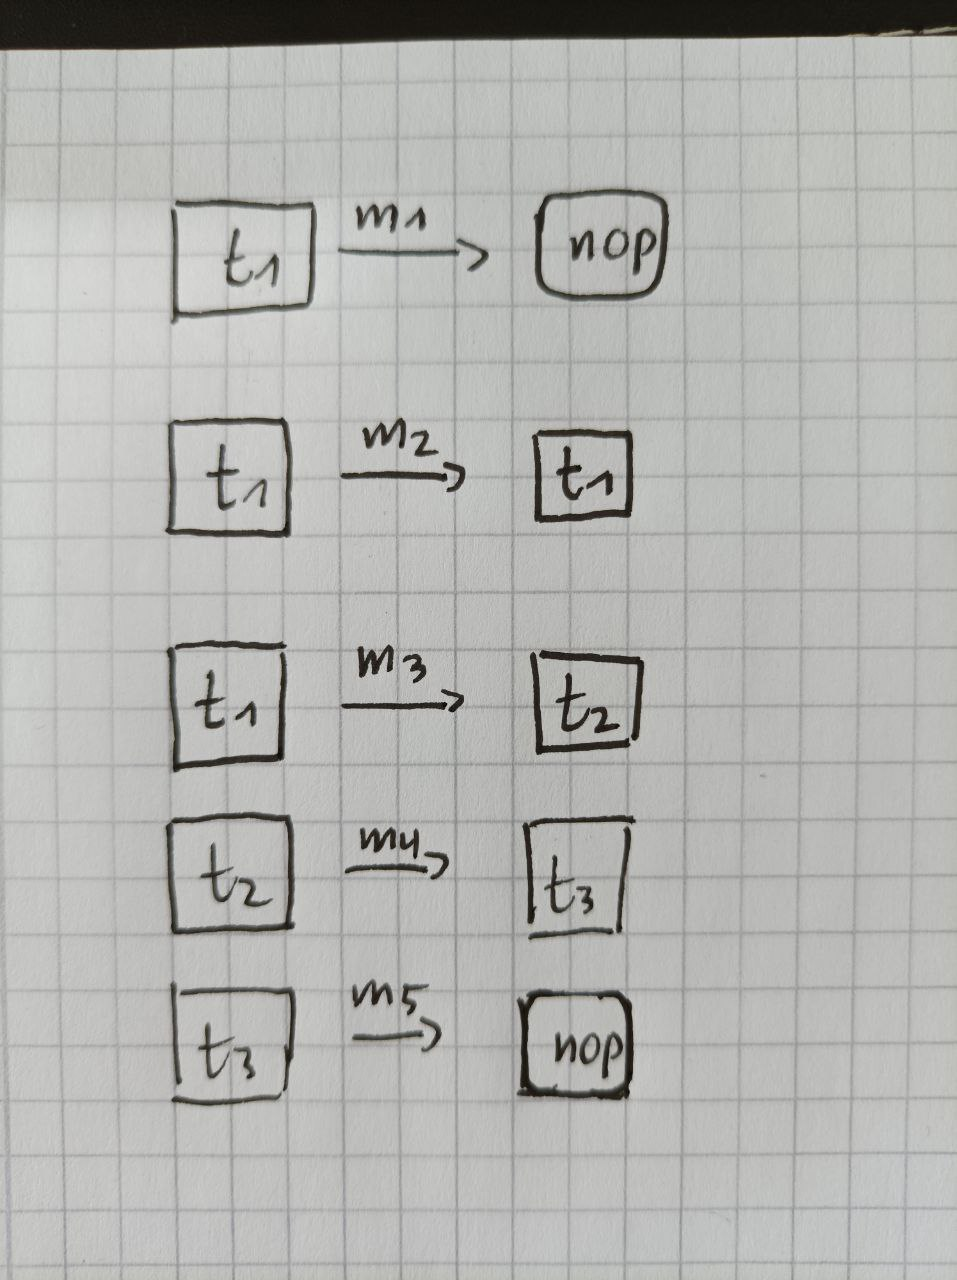
\includegraphics[width=0.5\textwidth]{images/prelim/improv_heuristic_pathological}
\end{figure}
Lastly, we implemented our heuristic search. While it does reuse the same heuristic, this algorithm achieves completeness by also valuing the number of applied methods so far. Let $n$ be a node with heuristic value $h$ and $r$ previously applied reductions to reach $n$. Then $n$ is guaranteed to be explored once all nodes with at most $h + r$ previously applied reductions have been explored. \\
All of this discussion so far has assumed sequential planners. We can easily extend the incompleteness of random and heuristic depth-first search to the parallel case. If we have an upper bound $p$ on the number of parallel processes we can build a domain as in figure \ref{figure: improv heuristic pathological} which does not induce 1 but $p$ endless looping opportunities that either trigger our heuristic or may simply be taken due to random chance. In this way, using parallelism does not get us to completeness but it does improve the our chances of at least 1 process taking the correct path.

\begin{comment}
- dfs: may find any solution but may also run into the wrong direction
- bfs: definitely complete, each node has an easy upper bound for when it is reached
- gbfs: may not find a plan at all if a heuristic is sufficiently pathological on an instance, leading into an endless loop
- astar: complete, distance travelled forces some bfs-like characteristics back into our exploration leading to completeness
\end{comment}
